% !TEX root = ../../thesis.tex

% Photo Yves Gellie
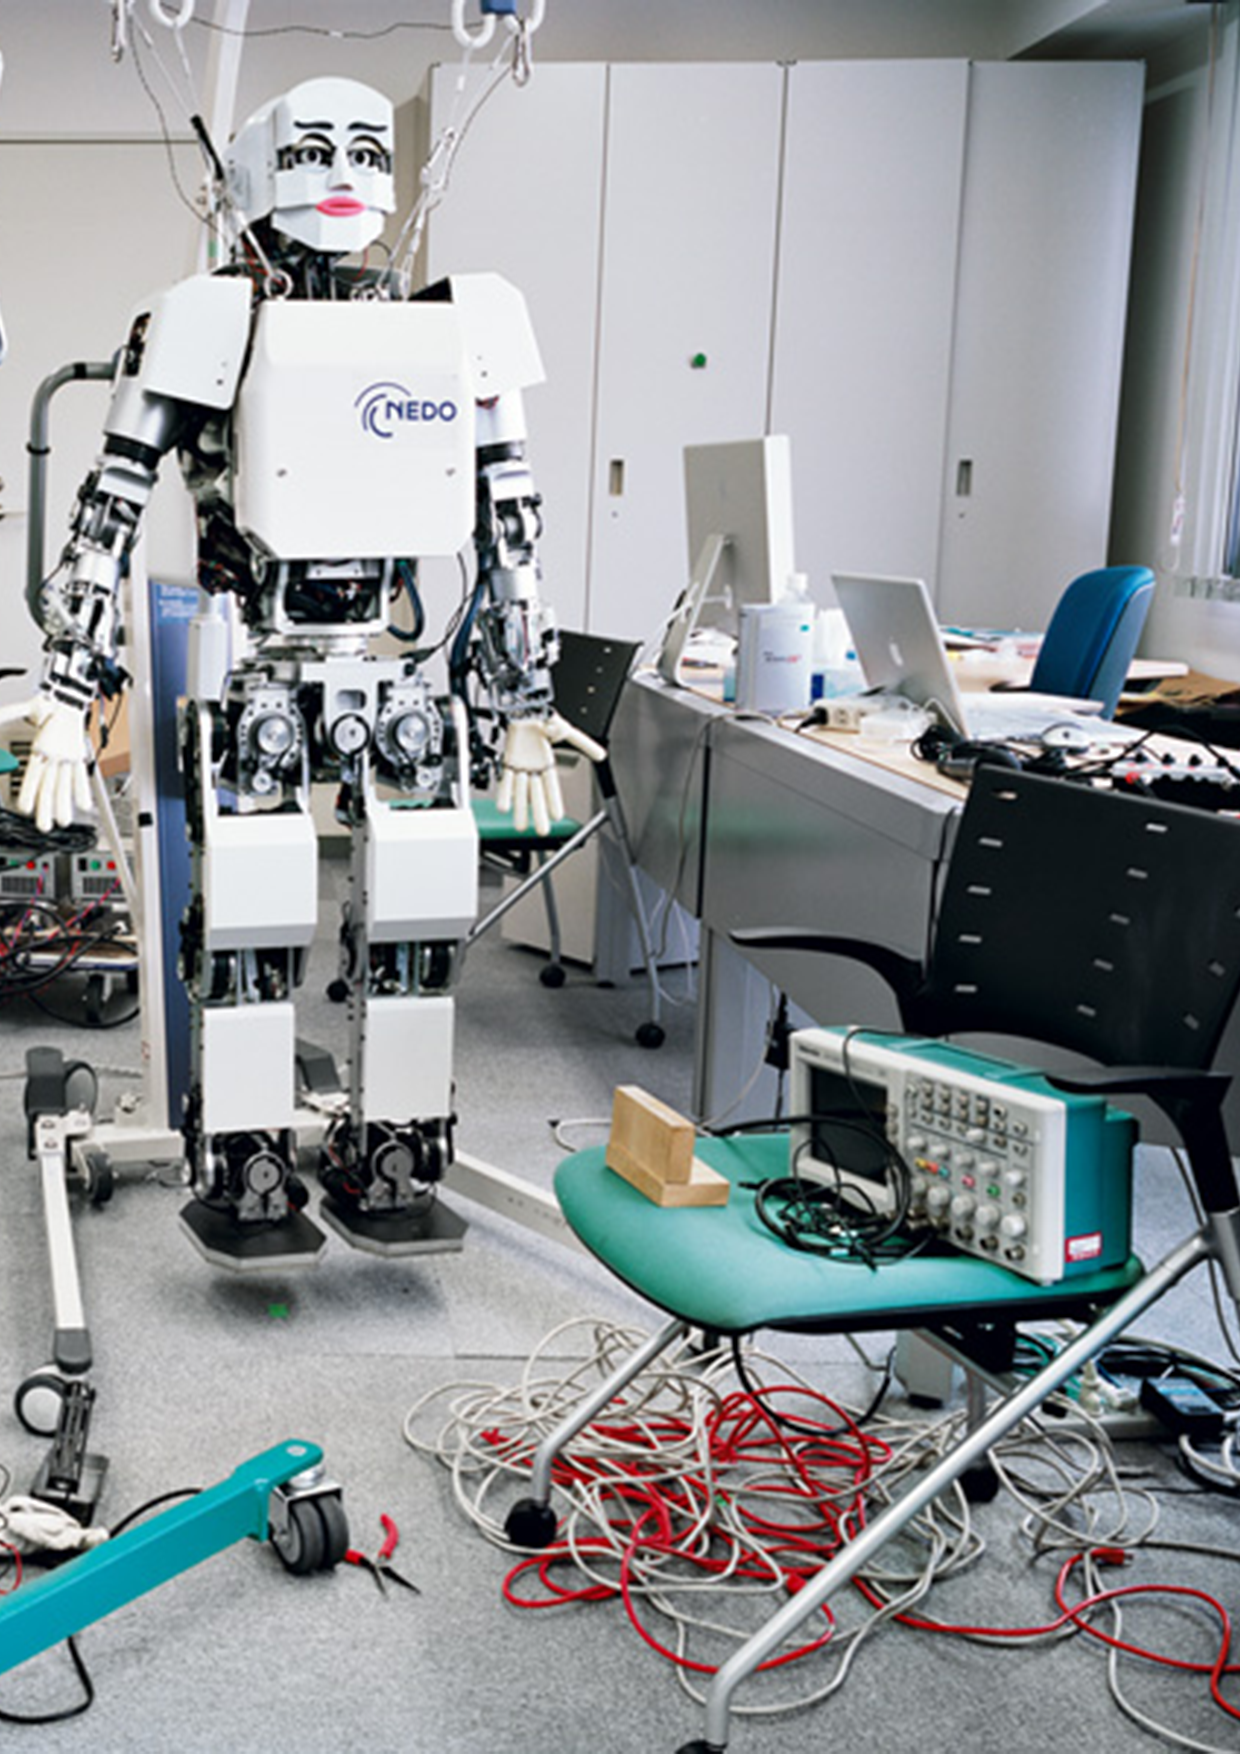
\includepdf{/Users/matthieulapeyre/Documents/phd_thesis/media/robot_setup.pdf}
\chapter{Review of experimental methods} % (fold)


\section{Simulation vs Real world} % (fold)


\begin{quotation}

First of all, we never actually produced a high-fidelity simulation. We made very simple simulations only. From them, we learned how to tune parameters. Then, we designed the real robots, without running full-blown optimizations. Rather, we used our intuition for a large number of decisions on design trade-offs, using lessons from the simple simulations combined with other limitations such as available motors etcetera. Then, we (again) used our intuition and large amount of experience to tune the robot’s controllers, and make design improvements, until it walked.

Even after obtaining a successful walking motion, we did not manage to create a simulation that walked successfully using the same controller parameters. We tried very hard with some of the best people, but we didn’t succeed. The reason was, I think, that our type of control (using the emergent behavior of a set of simple reflex-like controllers) was highly sensitive to hardware effects like friction. Normally, one uses a local joint controller to make the joint follow a desired trajectory independent of the exact amount of friction. The local controller “abstracts these hardware effects away”, if you know what I mean. This makes the behavior of the whole system quite predictable. However, in our robots, we did not have this kind of abstraction as we were not following trajectories, and thus a little bit of extra friction has an effect on the entire motion.

We did spend a long time making a high-fidelity model in Adams, and also using other methods, but eventually we gave up without success.

-- \textbf{Martijn Wisse - Associate professor at Delft University of Technology}

\end{quotation}

\section{Existing platforms} % (fold)

DarwinOP c'est comme Poppy mais pas forcement pensé pour explorer le role du corps.


\subsection{Humanoids and bipeds} % (fold)


\section{methods for building robots} % (fold)


\subsection{Actuation} % (fold)


\subsubsection{wire-driven} % (fold)

\subsubsection{Serie Elastic Actuator} % (fold)

\subsubsection{Pneumatic artificial muscle} % (fold)

\subsubsection{Hydraulic linear actuator} % (fold)


\section{Small humanoid robot} % (fold)
Robotis



\section{methods for dissemination and reproducibility} % (fold)

publish paper ...

Some info on a website ...

le gars du LAAS qui donne une VM

emails

open source (soft)

Matlab Exchange

Science community

Hack your PhD


\textbf{object}: Review of the robot, in particular biped.


\textbf{Conclusion}: There is no adapted or replicable platform. We need to create one.

